\chapter{Math: Probability and Statistics}

Crucial to the study of quantum physics, statistical physics, experiment, and
eventually lattice field theory is an understanding of probability and the
ability to understand statistics. These skills are actually quite important to
understand all modern science, not just physics, as well as in everyday
circumstances like politics.
You already have a rough idea of probability: It's a way of saying whether you
think something will happen or not, while in general signaling that you aren't
completely certain. We will now make these ideas precise.
Parts of this presentation follow selected parts
of Chapters~1 and~2 of Berg~\cite{berg_markov_2004}.


\section{Preliminaries}\label{sec:probprelim}


We will consider a {\it random variable}\index{random variable}\footnote{
We will try to denote random variables by capital letters.} $X$ which
has some possible {\it outcomes}\index{outcome} $x_i$. The random variable will take
one of the values in $x_i$, but we don't know for sure which one.
The set of all possible outcomes
\begin{equation}
  \Omega=\{x_1,x_2,...,x_n\},
\end{equation}
assuming there are $n\in\N$ possible outcomes, is called the {\it sample
space}\index{sample space}. If $\given\Omega\given$ is finite as in the above case, we
say that $X$ is {\it discrete}\index{discrete}. An {\it event}\index{event} $E$
is any subset of outcomes $E\subset\Omega$, and we assign it a {\it
probability}\index{probability} $\pr{E}$. Axiomatically speaking, the
probability has to fulfill two conditions:
\begin{enumerate}
  \item $\Forall E$, $0\leq\pr{E}\leq1$.
  \item $\pr{\Omega}=1$, i.e. the random variable $X$ needs to have some outcome
in $\Omega$. Another way to state this is that the probability of at least one
of the possibilities is 1.
\end{enumerate}

Pragmatically you can assign a probability by repeating some experiment $n$
times. If the event $E$ occurs $n_E$ times, then\footnote{Note that this limit 
is nontrivial since $n_E$ will in general change as $n$ increases.}
\begin{equation}\label{eq:freqdef}
  \pr{E}\equiv\lim_{n\to\infty}\frac{n_E}{n}.
\end{equation}
This method of assignment also gives a way to interpret
what a probability means; in particular $\pr{E}=0.3$ would mean that
if I repeat some experiment 10 times, I can expect to observe event
$E$ 3 times on average. This interpretation is called
the {\it frequentist}\index{frequentist approach} interpretation. We will
discuss another interpretation in the context of the 
{\it Bayesian}\index{Bayes!approach} approach in
\secref{sec:bayes}.
 
Alternatively, you can make some theoretical assignment of probabilities to
events. For instance when one tosses a coin, if one has no reason to believe the
coin is biased\footnote{One way of looking at this theoretical assignment
is that we have no reason to suppose heads is ``more likely" than tails,
i.e. there is no reason to prefer heads to tails. 
We call this the {\it principle of insufficient reason}\index{principle!insufficient reason}.
This approach to probability
assignment can be generalized to an arbitrary $n$-state system, which leads
to the uniform distribution.}, it must be that
\begin{equation}
\pr{\text{heads}}=\pr{\text{tails}}=\frac{1}{2}.
\end{equation}
This theoretical assignment is nice, but it should eventually be checked against
some observation or measurement as well.
In the case that $|\Omega|<\infty$,
we might say that the probability of event $E$ is $\pr{E}=|E|/|\Omega|$. In
this instance, we say that the probability is {\it uniform}
\index{PDF!uniform} since every point in the sample space is equally likely. 


Sometimes the cardinality of $\Omega$ is uncountably infinite. For instance you
may ask something like: What is the probability that a particle in this gas has
a speed between $v_1$ and $v_2$? In this case, the sample space is
\begin{equation}
  \Omega=\{x\suchthat0\leq x\leq c\},
\end{equation}
where $c$ is the speed of light.
In such a case we speak of a {\it continuous} random variable $X$.
The probability that $X$ takes any one particular value in $\Omega$ is
zero\footnote{Intuitively you could ask yourself: What is the probability that
my speed is exactly $\pi$ to all infinitely many digits? When checking against
experiment, you will never be able to resolve all infinitely many digits, so at
best you must specify a range corresponding to the resolution of your
instrument. In formal mathematical language, we require $\Omega$ to be
{\it measurable}.}.
We can only assign
sensible probabilities to subsets of $\Omega$ of uncountably infinite
cardinality. In the above
case, this corresponds to the range of velocities between $v_1$ and $v_2$.
The probability that $X$ takes a value in the small range of velocities $\dd x$
is denoted
\begin{equation}
   \pr{X\in[x,x+\dd x]}=\dd{x}f(x),
\end{equation}
and hence for continuous random variables, the probability must instead
fulfill the properties
\begin{enumerate}
  \item  $0\leq\dd{x}f(x)\leq 1$ and
  \item $\int_{x\in\Omega}\dd{x}f(x)=1$.
\end{enumerate}
In general for some integrable function 
$f:\R\to\R$, we assign a 
probability that $X$ lies in the interval $[a,b]$ by
\begin{equation}
  \label{eq:cpr}
  \pr{X\in[a,b]}=\int_a^b\dd{x}f(x).
\end{equation}
For the remainder of this chapter, we will
only be concerned with continuous random variables, and we will simply call
them random variables.
The function $f$ is called the {\it probability distribution function} 
(PDF)\index{PDF}; meanwhile the {\it cumulative distribution function} 
(CDF) is the function\index{CDF} $F(x)$ given by
\begin{equation}
  F(x)\equiv \pr{X<x}=\int_{-\infty}^x\dd{t}f(t).
\end{equation}
\begin{example*}{}{}
Two examples of important probability distributions include the {\it Gaussian}
or {\it normal} distribution,\index{PDF!normal}
\begin{equation}
  \gau(x,\hat{x},\sigma)\equiv\frac{1}{\sigma\sqrt{2\pi}}
  \exp\Bigg(-\frac{(x-\hat{x})^2}{2\sigma^2}\Bigg)
\end{equation}
where $\sigma$ is the standard deviation of the distribution and $\hat{x}$ is 
the mean, and the {\it Cauchy} \index{PDF!Cauchy} distribution,
\begin{equation}
  \cau(x,\alpha)\equiv\frac{\alpha}{\pi\big(\alpha^2+x^2\big)}.
\end{equation}
I will refer to these special PDFs later, particularly the normal distribution.
I'll call their CDFs $\Gau$ and $\Cau$, respectively.   
\end{example*}

Now that we know what probabilities and PDFs are, we can start thinking about
ways to characterize them. For example we can think about typical values taken
by a random variable from some distribution. We can get some information
from the mean and variance of a distribution. These are
both special cases of a more general concept.
In particular, let $n\in\N$.
  The {\it $n\nth$ moment} \index{moment}of the distribution $f(x)$ is
  \begin{equation}\label{dfn:mom}
    \ev{X^n}=\int_{-\infty}^\infty\dd{x}x^nf(x).
  \end{equation}

The mean and variance are the special cases $\hat{x}=\ev{X}$ and 
$\sigma^2=\ev{(X-\hat{x})^2}$. Sometimes we call the mean the {\it expected
value} and sometimes we denote the variance $\variance$. Note that not all 
probability distributions have well-defined moments. The Cauchy distribution is
very ill-behaved in this regard, since its $n\nth$ moment diverges
$\Forall n\in\N$.
Generally in the lab, one draws random variables from distributions
about which one has no a priori knowledge. Therefore in principle one
doesn't know the true moments these distributions. The
definition \eqref{dfn:mom} suggests a way to estimate them. 
Suppose you draw a sample $X_1,...,X_N$:
  An {\it estimator}\index{estimator} of the $n\nth$ moment is
  \begin{equation}
    \bar{X}^n\equiv\frac{1}{N}\sum_{i=1}^N X_i^n.
  \end{equation}
In the case $n=1$ we obtain the ordinary arithmetic average.
We use the hat to distinguish true values from estimators, which will
generally be denoted with a bar. For estimators of moments besides the
mean, we must be more careful; this is discussed in \secref{sec:bias}.

Consider two intervals $[a,b]$ and $[c,d]$ and two random variables
$X$ and $Y$ drawn from PDFs $f$ and $g$, respectively. Then $X$ and $Y$ are
said to be {\it independent}\index{random variable!independent} if
\begin{equation}\label{dfn:ind}
  \pr{X\in[a,b]\text{ and }Y\in[c,d]}=\int_a^b\int_c^d\dd{x}\dd{y}f(x)\,g(y)
\end{equation}
Hence we see that the {\it joint PDF}\index{PDF!joint} of $X$ and $Y$ 
is $f(x)g(y)$. On the other hand, we say $X$ and $Y$ are {\it uncorrelated} 
\index{random variable!uncorrelated} if
\begin{equation}
  \ev{XY}=\ev{X}\ev{Y},
\end{equation}
The {\it covariance}\index{covariance}
\begin{equation}\label{dfn:cov}
  \Cov[X,Y]\equiv\ev{XY}-\ev{X}\ev{Y}
\end{equation}
can be used to give a measure of how correlated $X$ and $Y$ are, or
one can use the {\it correlation}\index{correlation}
\begin{equation}\label{dfn:cor}
  \rho(X,Y)=\frac{\Cov[X,Y]}{\sigma_X\sigma_Y}.
\end{equation}
So equivalently we say $X$ and $Y$ are correlated if $\rho(X,Y)=0$.
It's worth emphasizing that if $X$ and $Y$ are independent,
it follows that they are uncorrelated. This can be seen by applying
definition \eqref{dfn:mom} to the random variable $XY$, then using
definition \eqref{dfn:ind}. However if $X$ and $Y$ are
uncorrelated, {\it they can still be dependent}.
\begin{example*}{}{}
  Here's an extreme example by Cosma Shalizi~\cite{cosma_indep}. 
Let $X$ be uniformly distributed
  on [-1,1] and let $Y=|X|$. Then clearly $Y$ depends on $X$. However it 
  is easy to see that $Y$ is uniform on [0,1] and $\ev{XY}=0=\ev{X}\ev{Y}$. 
  Hence $X$ and $Y$ are not correlated.
\end{example*}

The next two propositions show us how to add expectation values and
random variables. Let $X$ and $Y$ be independent random variables 
drawn from PDFs $f$ and $g$, respectively.
\begin{proposition}{}{}
  Let $a,b\in\R$ be constants. Then
  $$\ev{aX+bY}=a\ev{X}+b\ev{Y}.$$
  \begin{proof}
    Since $X$ and $Y$ are independent, their joint PDF is $fg$. Then
    \begin{equation*}
      \begin{aligned}
      \ev{aX+bY}&=\int\dd{x}\dd{y}(ax+by)f(x)g(y)\\
                &=a\int\dd{x}\dd{y}x\,f(x)g(y)+
                 b\int\dd{x}\dd{y}y\,f(x)g(y)\\
                &=a\int\dd{x}x\,f(x)+b\int\dd{y}y\,g(y)\\
                &=a\ev{X}+b\ev{Y}.
      \end{aligned}
    \end{equation*}
  \end{proof}
\end{proposition}

\begin{proposition}{}{addvars}
  The PDF of the random variable $Z=X+Y$ is given by the convolution
  \begin{equation*}
    h(z)=\int_{-\infty}^\infty\dd{x}f(x)g(z-x)
  \end{equation*}
  \begin{proof}
    The CDF of $Y$ is, according to \equatref{dfn:ind},
    \begin{equation*}
      H(y)=\int_{x+y\leq z}\dd{x}\dd{y}f(x)g(y)
          =\int_{-\infty}^\infty\dd{x}f(x)\int_{-\infty}^{z-x}
            \dd{y}g(y).
    \end{equation*}
    The PDF $h$ follows from the Fundamental Theorem of Calculus:
    \begin{equation*}
      h(z)=\dv{H}{z}=\dv{H}{(z-x)}
          =\int_{-\infty}^\infty\dd{x}f(x)g(z-x).
    \end{equation*}
  \end{proof}
\end{proposition}

A sequence $\{X_N\}$ of random variables 
\index{converge!in probability}{\it converges in probability}
toward the random variable $X$ if $\Forall\epsilon>0$ 
\begin{equation}
  \lim_{N\to\infty}\pr{|X_N-X|>\epsilon}=0,
\end{equation}
and we write
\begin{equation}
  X_N\xrightarrow{\text{P}}X.
\end{equation}
The sequence converges to $X$ 
\index{converge!almost surely}{\it almost surely} if
\begin{equation}
  \lim_{N\to\infty}\pr{X_N=X}=1,
\end{equation}
and in this case we write
\begin{equation}
  X_N\xrightarrow{\text{AS}}X.
\end{equation}

\index{Chebyshev's inequality}
\begin{theorem}{Chebyshev's inequality}{}
  \index{Chebyshev's inequality}
  Let $X$ be drawn from a PDF with mean $\hat{x}$ and variance
  $\sigma^2$ and let $a>0$. Then
  \begin{equation*}
    \pr{|X-\hat{x}|>a\sigma}<a^{-2}.
  \end{equation*}
  \begin{proof}
    Let $T=(X-\hat{x})^2$ be a new random variable with PDF $g$. Then
    \begin{equation*}
      \pr{|X-\hat{x}|>a\sigma}=\pr{T>a^2\sigma^2}
                              =\int_{a^2\sigma^2}^\infty\dd{t}g(t)
    \end{equation*}
    But
    \begin{equation*}
      \begin{aligned}
        \sigma^2&=\int_{0}^\infty\dd{t}t\,g(t)
                =\Bigg(\int_0^{a^2\sigma^2}
                     +\int_{a^2\sigma^2}^\infty\Bigg)\dd{t}t\,g(t)\\
                &\geq\int_{a^2\sigma^2}^\infty\dd{t}t\,g(t)
                >a^2\sigma^2\int_{a^2\sigma^2}^\infty\dd{t}g(t)
                =a^2\sigma^2\pr{T>a^2\sigma^2}.
      \end{aligned}
    \end{equation*}
   Dividing through by $a^2\sigma^2$ completes the proof.
  \end{proof} 
\end{theorem}
Chebyshev's inequality tells you that large deviations from the mean are
unlikely. Intuitively you expect that as the number of measurements
increases, the sample average tends toward the true mean. This is
called the {\it Law of Large Numbers}\index{LLN}
(LLN). To prove it, we set up as follows: Let $X_1,...,X_N$ be a sequence 
of random variables drawn from a PDF
with mean $\hat{x}$ and variance $\sigma^2$.
\begin{theorem}{Weak LLN}{}
  $$
    \bar{X}\xrightarrow{\text{P}}\hat{x}.
  $$
  \begin{proof} Our proof will rely on Chebyshev's inequality, so we will
    first need to compute the mean and variance of the distribution of
    $\bar{X}$. All the $X_i$ are drawn from the same PDF, so
    $$
      \ev{\bar{X}}=\frac{1}{N}\sum_{i=1}^N\ev{X_i}
                  =\frac{N\hat{x}}{N}=\hat{x}.
    $$
    Meanwhile the variance of the distribution of $\bar{X}$ is
    $$
      \sigma^2_{\bar{X}}
      =\variance\sum_{i=1}^N \frac{X_i}{N}
      =\sum_{i=1}^N\frac{\sigma^2}{N^2}
      =\frac{\sigma^2}{N}.
    $$
    Now let $\epsilon>0$. Then $\exists\,a>0$ with 
    $\epsilon=a\,\sigma_{\bar{X}}$. Hence by Chebyshev's
    inequality we have
    $$
      \lim_{N\to\infty}\pr{|\bar{X}-\hat{x}|>\epsilon}
       \leq\lim_{N\to\infty}\frac{\sigma^2_{\bar{X}}}{\epsilon^2}
       =\lim_{N\to\infty}\frac{\sigma^2}{N\epsilon^2}=0.
    $$
    The probability can't be less than 0, so we're done.
  \end{proof}
\end{theorem}
The above proof relies on the PDF having a finite
variance. As it turns out, the Weak LLN is true
even when the variance is infinite! This can be proved
using characteristic functions. But since we don't introduce characteristic
functions until \secref{sec:CLT}, and since we assume in practice
that our data are drawn from PDFs with finite variance anyway,
we direct the reader elsewhere. For example, a proof can be
found on Wikipedia~\cite{Wiki_LLN}.

For completeness we also list the Strong LLN, but without proof. 
Like the Weak LLN, the Strong LLN is true even when the PDF variance
is infinite.

\begin{theorem}{Strong LLN}{}
  $$
    \bar{X}\xrightarrow{\text{AS}}\hat{x}.
  $$
\end{theorem}

Also in this section we list a sometimes useful fact about CDFs, which is
for example helpful in interpreting the results of some statistical
tests. (See e.g. \thmref{thm:gaudif}.) 

\begin{proposition}{}{}
  If a random variable $X$ is distributed according to the PDF $f$, then
  the corresponding CDF $F$ is distributed uniformly in [0,1].
  \begin{proof}
    If a random variable $Y$ is distributed uniformly in [0,1], then
    by definition we have $\Forall r\in [0,1]$
    $$
      \pr{0\leq Y\leq r}=r.
    $$
    So all we have to do is show that $F(X)$ behaves like $Y$. To that end,
    let $r\in[0,1]$ and define $X^*\in\R$ by
    $$
      r=\int_\infty^{X^*}\dd{s}f(s).
    $$
    Then
    $$
      \pr{0\leq F(X)\leq r}
      =\pr{-\infty\leq X\leq X^*}
      =\int_{-\infty}^{X^*}\dd{s}f(s)
      =r.
    $$
  \end{proof}
\end{proposition}

\section{The normal distribution}
\index{PDF!normal}
Now we're going to focus on results about the normal distribution specifically.
This first proposition will aid us in some of the calculations.

\begin{proposition}{}{gauss}
  Let $\alpha>0$. Then
  \begin{equation*}
    \int_{-\infty}^\infty\dd{x}e^{-\alpha x^2}=\sqrt{\frac{\pi}{\alpha}}.
  \end{equation*}
  \begin{proof}
    The trick is to just square the LHS:
    \begin{equation*}\begin{aligned}
      \left(\int_{-\infty}^\infty\dd{x}e^{-\alpha x^2}\right)^2
      &=\int_{-\infty}^\infty\int_{-\infty}^\infty\dd{x}\dd{y}
        e^{-\alpha(x^2+y^2)}\\
      &=\int_0^\infty \dd{r}r\int_0^{2\pi}\dd{\theta}e^{-\alpha r^2}\\
      &=\frac{\pi}{\alpha}.
    \end{aligned}\end{equation*}
  \end{proof}
\end{proposition}

For the next result 
let $X_1$ and $X_2$ be two independent random variables drawn from normal
distributions with respective means $\hat{x}_1$ and $\hat{x}_2$ and
standard deviations $\sigma_1$ and $\sigma_2$. 
\begin{proposition}{}{addgauss}
  The random variable $Y=X_1+X_2$ is normally distributed with mean
  $\hat{x}_1+\hat{x}_2$ and variance $\sigma_1^2+\sigma_2^2$.
  \begin{proof}
    By \propref{prp:addvars}, the sum $Y$ has the distribution
    \begin{equation*}
      g(y)=\frac{1}{2\pi\sigma_1\sigma_2}
           \int_{-\infty}^\infty\dd{x}\exp\left[
             -\frac{(x-\hat{x}_1)^2}{2\sigma_1^2}
             -\frac{(y-x-\hat{x}_2)^2}{2\sigma_2^2}\right].
    \end{equation*}
    Pull everything out of the integral that doesn't depend on $x$,
    then complete the square with what's left over.
    One obtains for $g(y)$
    $$
      \frac{1}{2\pi\sigma_1\sigma_2}
           \exp\left[-\frac{(y-\hat{x}_1-\hat{x}_2)^2}
                      {2(\sigma_1^2+\sigma_2^2)}\right]
           \int_{-\infty}^\infty\dd{x}
           \exp\left[-\frac{\sigma_1^2+\sigma_2^2}
                     {2\sigma_1^2\sigma_2^2}(x+C)^2\right],
    $$
    where $C$ is just a bunch of stuff that doesn't depend on $x$.
    Therefore you can make the substitution $u=x+C$ with $\dd u=\dd x$ and
    carry out the new integral using \propref{prp:gauss}.
    The result is
    \begin{equation*}
      g(y)=\frac{1}{\sqrt{2\pi(\sigma_1^2+\sigma_2^2)}}
           \exp\left[-\frac{(y-\hat{x}_1-\hat{x}_2)^2}
                      {2(\sigma_1^2+\sigma_2^2)}\right].
    \end{equation*}
  \end{proof}
\end{proposition}

Since the normal distribution is so important, so must be its CDF.
Unfortunately the integral of the normal PDF is {\it non-elementary};
\index{non-elementary} that is, it can't be expressed in terms of 
polynomials or standard
functions like $\sin$, $\cos$, or $\exp$. Therefore we give a name
to this special function.
The {\it error function}\index{error function} is
\begin{equation}
  \erf(x)\equiv\frac{2}{\sqrt{\pi}}\int_0^x\dd{t}e^{-t^2}.
\end{equation}
Then we can write the Gaussian CDF with mean 0 as
\begin{equation}
  \label{eq:gaussCDF}
  \Gau(x,0,\sigma)=\frac{1}{\sqrt{2\pi}\sigma}
                   \int_{-\infty}^x\dd{t}e^{-t^2/2\sigma^2}
                  =\frac{1}{2}+\frac{1}{2}
                   \erf\left(\frac{x}{\sqrt{2}\sigma}\right).
\end{equation}
Now we can list some pretty powerful applications of the normal distribution.
For instance one often must compare two empirical estimates of some mean.
Usually these estimates are different, and one might wonder whether this
disparity is real or just plain unlucky. More precisely:
\index{Gaussian difference test}
\begin{theorem}{Gaussian difference test}{}\label{thm:gaudif}
  Suppose $\bar{X}$ and $\bar{Y}$ are correct estimates of 
  some expectation
  value, i.e. they are normally distributed with the same mean, and call
  their respective standard deviations $\sigma_X$ and
  $\sigma_Y$. Then the probability that $\bar{X}$ 
  and $\bar{Y}$ differ by at least $D$ is
  \begin{equation*}
    \pr{|\,\bar{X}-\bar{Y}|>D}=1-\erf\left(\frac{D}
       {\sqrt{2(\sigma_X^2+\sigma_Y^2)}}\right).
  \end{equation*}
  \begin{proof}
    From \propref{prp:addgauss}, the random variable
    $\bar{X}-\bar{Y}$ is normally distributed with mean 0 
    and variance $\sigma_D^2=\sigma_X^2+\sigma_Y^2$. Therefore by
    \equatref{eq:gaussCDF}, the probability that $\bar{X}$ and 
    $\bar{Y}$ are at most $D$ apart is
    \begin{equation*}
      \begin{aligned}
        \pr{|\,\bar{X}-\bar{Y}|<D}
            &=\pr{-D<\bar{X}-\bar{Y}<D}\\
            &=\Gau(D,0,\sigma_D)-\Gau(-D,0,\sigma_D)\\
            &=1-2\Gau(-D,0,\sigma_D)\\
            &=\erf\left(\frac{D}{\sqrt{2}\sigma_D}\right).
      \end{aligned}
    \end{equation*}
    And of course, $\pr{|\,\bar{X}-\bar{Y}|>D}
     =1-\pr{|\,\bar{X}-\bar{Y}|<D}$.
  \end{proof}
\end{theorem}
In other words, the above theorem gives the probability that the
observed difference $|\bar{X}-\bar{Y}|$ is due to chance. This probability
is called the \index{q-value}{\it q-value}. In practice one sets some 
threshold on $q$ below which one investigates further whether the 
underlying distributions of the estimates are different. Often one 
takes the threshold as 0.05.

\section{The central limit theorem}\label{sec:CLT}

Let $X$ and $Y$ be real random variables. Then we can construct a
complex random variable $F=X+iY$, and its expectation value will be
\begin{equation}
  \ev{F}=\ev{X}+i\ev{Y}.
\end{equation}
This allows us to speak sensibly about Fourier transformations of
PDFs. In particular let $X$ be drawn from the PDF $f$.
The {\it characteristic function}
\index{random variable!characteristic function} of $X$ is
\begin{equation}
  \phi(t)\equiv\ev{e^{itX}}=\int_{-\infty}^\infty\dd{x}e^{itx}f(x).
\end{equation}
Knowing the characteristic function $X$ is equivalent to knowing its PDF;
this is because we can take the inverse Fourier transformation
\begin{equation}
  f(x)=\frac{1}{2\pi}\int_{-\infty}^\infty\dd{t}e^{-itx}\phi(t),
\end{equation}
which follows from the Dirac $\delta$-function. The derivatives of the
characteristic function are easily calculated to be
\begin{equation}
  \phi^{(n)}(t)=i^n\int_{-\infty}^\infty\dd{x}x^ne^{itx}f(x);
\end{equation}
therefore
\begin{equation}
  \phi^{(n)}(0)=i^n\ev{X^n}.
\end{equation}
If $|f(x)|$ falls off faster than $x^m$ for any $m\in\mathbb{Z}$, then
it follows from the above equation that all moments exist, and the
characteristic function is analytic in $t$ about $t=0$.

These are some neat properties of characteristic functions; however
our main use for them is summarized in the next proposition.
\begin{proposition}{}{addchars}
  The characteristic function of a sum of independent random variables equals 
  the product of their characteristic functions.
  \begin{proof}
    Let $X_1$,...,$X_N$ be drawn from PDFs $f_1$,...,$f_N$ with
    corresponding characteristic functions $\phi_1,...,\phi_N$, and
    let $Y=\sum_j X_j$. Then using the definition of the characteristic
    function we obtain
    $$
      \phi_Y(t)=\ev{e^{it\sum_j X_j}}=\ev{\prod_{j=1}^N e^{it X_j}}\\
               =\prod_{j=1}^N \ev{e^{it X_j}}=\prod_{j=1}^N\phi_j(t),
    $$
    where we used independence for the third equality.
  \end{proof}
\end{proposition}
Now suppose you're an experimenter taking independent measurements of 
some observable. Furthermore suppose you don't know anything about the 
observable, except that it comes from some distribution with finite variance.
The central limit theorem (CLT) says that armed with this information alone, 
you know that the sample mean will be normally distributed about
the true mean. Here is the precise statement. 
\begin{theorem}{Central limit theorem}{}
  \index{CLT}
  Let $X_1,...,X_N$ be $N$ independent random variables drawn from PDF $f$.
  Suppose further that $f$ has mean $\hat{x}$ and variance $\sigma^2$. 
  Then the PDF of the estimator $\bar{X}$ converges to 
  $\gau(\bar{x},\hat{x},\sigma/\sqrt{N})$.
  \begin{proof}
    What we're going to do is look at the characteristic function 
    $\phi_S$ of the random variable
    $$
      S\equiv\bar{X}-\hat{x}=\frac{X_1+...+X_N-N\hat{x}}{N}.
    $$
    If we can show that $\phi_S$ converges to the characteristic function
    corresponding to $\gau(s,0,\sigma/\sqrt{N})$, then we are finished.
    In order to show this, we first need the characteristic function for
    the distribution $\gau(s,0,\sigma/\sqrt{N})$. By completing the
    square and using \propref{prp:gauss}, we find 
    \begin{equation*}
      \begin{aligned}
        \phi_{\text{gau}}
            &=\frac{1}{\sigma}\sqrt{\frac{N}{2\pi}}\int_{-\infty}^\infty\dd{s}
              e^{its}\exp\left[-\frac{s^2N}{2\sigma^2}\right]\\
            &=\frac{1}{\sigma}\sqrt{\frac{N}{2\pi}}
              \exp\left[-\frac{\sigma^2t^2}{2N}\right]
              \int_{-\infty}^\infty\dd{s}
              \exp\left[-\frac{N}{2\sigma^2}(s-C)^2\right]\\
            &=\exp\left[-\frac{\sigma^2t^2}{2N}\right],
      \end{aligned}
    \end{equation*}
    where $C$ is a number that doesn't depend on $s$. It remains to show 
    $\phi_S=\phi_{\text{gau}}$. By \propref{prp:addchars} we have
    $$
      \phi_S(t)=\phi_{\frac{1}{N}\sum X_i-\hat{x}}(t)
               =\left[\phi_{X-\hat{x}}\left(\frac{t}{N}\right)\right]^N,
    $$
    where $\phi_{X-\hat{x}}$ is the characteristic function corresponding
    to the random variable $X-\hat{x}$. Call its PDF $g$. From the
    properties of $f$, we know that $g$ has mean 0 and variance $\sigma^2$.
    Therefore by expanding $\phi_S$ about $t=0$ and using the 
    definition \eqref{dfn:mom}, we find
    $$
      \phi_S(t)=\left[1-\frac{\sigma^2t^2}{2N^2}
             +\order{\frac{t^3}{N^3}}\right]^N
               =\exp\left[-\frac{\sigma^2t^2}{2N}\right]
             +\order{\frac{t^3}{N^2}},
    $$
    as desired.
  \end{proof}
\end{theorem}
Since the variance of the estimator $\bar{X}$ tends to 0 for large $N$,
it follows that the sample mean converges to the true mean $\hat{x}$.
In particular for large $N$, we expect the true mean to be within
$\sigma/\sqrt{N}$ of the estimator roughly 68\% of the time.
\tabref{tab:normal} gives the area under a Gaussian curve 
for different numbers of standard deviations away from the mean. 

\begin{table}
\centering
\caption{Table of areas under the curve for the normal distribution.
The last column gives the probability that a random variable 
drawn from the distribution falls at least the given number of error bars 
away from the mean.}
\begin{tabularx}{\linewidth}{cCr}
\hline\hline
Number of $\sigma$ from $\hat{x}$ & Area under curve & About 1 in ...\\
\hline
1 & 0.682 689 49 & 3\\
2 & 0.954 499 74 & 22\\
3 & 0.997 300 20 & 370\\
4 & 0.999 936 66 & 15 787\\
5 & 0.999 999 43 & 1 744 278\\
\hline\hline
\end{tabularx}
\label{tab:normal}
\end{table}

\section{Bias}\label{sec:bias}

For this section consider independent random variables $X_1,...,X_N$ 
drawn from a distribution with mean $\hat{x}$ and variance $\sigma^2$. 
Earlier we recovered the familiar estimator for the mean, which was
just the ordinary arithmetic average. But what about an estimator for 
the variance? Naively one might write
\begin{equation}\label{eq:bad}
  \bar{\sigma}^2_{\text{biased}}=\frac{1}{N}\sum_{i=1}^N(X_i-\bar{X})^2;
\end{equation} 
While we expect this estimator to converge\footnote{An estimator that
converges to the correct result as $N\to\infty$ is
{\it consistent}\index{consistent}. Note that unbiased and consistent
do not mean the same thing; in particular $\bar{\sigma}^2_{\text{biased}}$
is consistent but biased.} to the
exact result in the limit $N\to\infty$, it disagrees with
$\sigma^2$ for small $N$. Most glaringly when $N=1$, the
estimator is zero, regardless of the exact result.
\index{bias}
An estimator is said to be {\it biased} when its expectation value
does not agree with the exact result. The difference between the
expectation value of the estimator and the exact result is
correspondingly called the {\it bias}. When they agree, we say
the estimator is {\it unbiased}.
\begin{proposition}{}{stdev}
  An unbiased estimator of the variance is
  $$
    \bar{\sigma}^2=\frac{1}{N-1}\sum_{i=1}^N(X_i-\bar{X})^2.
  $$
  \begin{proof}
  To construct an unbiased estimator of the variance,
  we'll determine the bias of the estimator, then remove it. Note
  \begin{equation*}
    \ev{\bar{\sigma}^2_{\text{biased}}}=\frac{1}{N}\sum\limits_{i=1}^N
      \left(\ev{X_i^2}-2\ev{X_i\bar{X}}+\ev{\bar{X}^2}\right).
  \end{equation*}
  Let us analyze the above equation term by term. Since the random
  variables $X_i$ are drawn from the same distribution, the first term
  is an unbiased estimator of $\ev{X^2}$ for each $i$. Next the
  second term can be rewritten as
  \begin{equation*}
    \begin{aligned}
    \ev{X_i\bar{X}}&=\frac{1}{N}\left(\ev{X_i^2}+
                     \sum_{j\suchthat j\neq i}\ev{X_iX_j}\right)\\
                   &=\frac{1}{N}\left(\ev{X^2}+(N-1)\ev{X}^2\right)\\
                   &=\frac{1}{N}\left(\ev{X^2}-\ev{X}^2\right)+\ev{X}^2\\
                   &=\frac{\sigma^2}{N}+\hat{x}^2,
    \end{aligned}
  \end{equation*}
  where in the second line we used the independence of the $X_i$. Finally
  for the last term we have
  $$
    \ev{\bar{X}^2}=\ev{\frac{1}{N^2}\sum_{i,j}X_iX_j}
        =\frac{1}{N^2}\left(N\ev{X^2}+\sum_{i,j\suchthat i\neq j}\hat{x}^2\right)
        =\frac{\sigma^2}{N}+\hat{x}^2,
  $$
  where we again used independence in the second equality. Plugging
  everything into $\ev{\bar{\sigma}^2_{\text{biased}}}$ gives
  \begin{equation*}
      \ev{\bar{\sigma}^2_{\text{biased}}}
        =\frac{1}{N}\sum_{i=1}^N
          \left(\ev{X^2}-\frac{\sigma^2}{N}-\hat{x}^2\right)
        =\left(\frac{N-1}{N}\right)\sigma^2.
  \end{equation*}
  This equation shows us the bias is $-\sigma^2/N$. Therefore according
  to this equation, an unbiased estimator of the variance is
  $$
    \bar{\sigma}^2=\left(\frac{N}{N-1}\right)\bar{\sigma}_\text{biased}^2
                  =\frac{1}{N-1}\sum_{i=1}^N(X_i-\bar{X})^2
  $$
  as we wished to show.
  \end{proof}
\end{proposition}
\vspace{1cm}
We saw that the bias of the naive variance estimator goes like $1/N$. 
So one might wonder: How much bias does one typically expect to encounter? 
Bias problems often appear whenever one wants to estimate some function 
of the mean $\hat{f}=f(\hat{x})$ that is not necessarily linear near the 
mean. One might be tempted to take the estimator
\begin{equation}
  \bar{f}_{\text{bad}}=\frac{1}{N}\sum_{i=1}^Nf_i,
\end{equation}
where $f_i\equiv f(X_i)$. However such an estimator is usually biased,
and even worse, we have in general that
\begin{equation}
  \lim_{N\to\infty}\bar{f}_\text{bad}\neq\hat{f}.
\end{equation}

\begin{example}{}{} Consider $N$ measurements of a random variable $X$ that
are drawn from a PDF with  $\hat{x}=0$, and suppose we are interested 
in estimating the function $f(x)=x^2$. If we try the bad estimator, we find
\begin{equation}
  \bar{f}_\text{bad}=\frac{1}{N}\sum_{i=1}^N X_i^2,
\end{equation}
which is guaranteed to be larger than 0 for each $i$, since $X_i=0$
with probability 0. In other words it is biased. For a more egregious example, 
we consider the piecewise function
\begin{equation*}
  f(x)=
  \begin{cases}
  0 & x=0, \\
  1 & \text{otherwise}.
  \end{cases}
\end{equation*}
In this example, clearly $\hat{f}=0$, but again since $X_i=0$ with probability
0 for each $i$, we will find
\begin{equation*}
  \lim_{N\to\infty}\bar{f}_\text{bad}=1.
\end{equation*}
\end{example}

An estimator that never converges to its true value is called
{\it inconsistent}; otherwise it is {\it consistent}.
\index{estimator!consistent}
So this bad estimator is not a consistent estimator. Note that a biased
estimator is not necessarily inconsistent; for instance the biased estimator
of the variance \equatref{eq:bad} is consistent. A consistent estimator
of $\hat{f}$ is
\begin{equation}\label{eq:consistentEstimator}
  \bar{f}=f(\bar{X}).
\end{equation} 
We can prove the consistency of $\bar{f}$ for a wide class of functions.
\begin{proposition}{}{bias}
  Suppose $f:\R\to\R$ has a convergent Taylor series 
  in a region about $\hat{x}$. If $\bar{X}$ maps to this region, 
  then $\bar{f}$ has bias of order $1/N$.
  \begin{proof}
    If we consider $f$ as a function of the ordinary variable $x$, we can
    expand it about $\hat{x}$ as
    $$
      f(x)=f(\hat{x})+f'(\hat{x})(x-\hat{x})
           +\frac{1}{2}f''(\hat{x})(x-\hat{x})^2
           +\order{(x-\hat{x})^3}.
    $$
    Since $\bar{X}$ maps to the region in which this expansion is valid,
    we can plug it into the above formula and find its expected value.
    This gives
    $$
      \ev{\bar{f}}-\hat{f}=f'(\hat{x})\ev{\bar{X}-\hat{x}}
           +\frac{1}{2}f''(\hat{x})\ev{(\bar{X}-\hat{x})^2}
           +\order{(\bar{X}-\hat{x})^3}.
    $$
    The LHS of this equation is the bias of $\bar{f}$. To simplify the
    RHS, note that by the CLT $\ev{\bar{X}-\hat{x}}=0$ and
    $\ev{(\bar{X}-\hat{x})^2}=\sigma^2/N$. Therefore
    $$
      \ev{\bar{f}}-\hat{f}=\frac{1}{2}f''(\hat{x})\frac{\sigma^2}{N}
                           +\order{\frac{1}{N^2}}.
    $$
  \end{proof}
\end{proposition}
According to the above proposition, the bias vanishes as $N\to\infty$, which
shows that $\bar{f}$ is consistent. For large $N$, $\bar{X}$ is very likely
to be close to $\hat{x}$ by the CLT, so \propref{prp:bias} will 
essentially hold whenever $N$ is large and $f$ is a nice enough function.
There is another important consequence to this proposition: the bias
decreases faster than the statistical error bar, which you will recall
goes like $1/\sqrt{N}$. Hence when $N$ becomes large enough, the bias
can be ignored.

\section{Error propagation and covariance}\label{sec:prop}
We will now reproduce the commonly used error propagation formula. We know
that if we have a smooth function of $N$ variables 
$f:\R^N\to\R$ we can Taylor expand
\begin{equation}
  f(x)=f(\hat{x})+\sum_{j=1}^N
        \pdv{f}{x_j}\Bigg|_{x=\hat{x}}(x_j-\hat{x}_j)
        +\order{x^2}
\end{equation}
where $x=(x_1,...,x_N)$ and $\hat{x}=(\hat{x}_1,...,\hat{x}_N)$. So if 
$|x-\hat{x}|$ is small enough, $f$ is a linear function of the components 
of $x$. This motivates the following situation: Suppose we have a set of 
$M$ random variables $Y_i$, each of which is a linear function of $N$ 
random variables $X_j$; i.e.
\begin{equation}\label{eq:lintran}
  Y_i=a_{i0}+\sum_{j=1}^N a_{ij}X_j.
\end{equation}
Then the mean is given by
\begin{equation}
  \hat{y}_i=\ev{Y_i}=a_{i\,0}+\sum_{j=1}^N a_{ij}\ev{x_j}
           =a_{i\,0}+\sum_{j=1}^N a_{ij}\hat{x}_j.
\end{equation}
Meanwhile the variance of $Y_i$ is given by
\begin{equation}\label{eq:linprop}
  \begin{aligned}
    \sigma^2_{Y_i}=\ev{(Y_i-\hat{y}_i)^2}
              &=\ev{\sum_{j=1}^N a_{ij}(X_j-\hat{x}_j)
                   \sum_{k=1}^N a_{ik}(X_k-\hat{x}_k)}\\
              &=\sum_{j=1}^N a_{ij}^2\ev{(X_j-\hat{x}_j)^2}
               +\sum_{j\neq k}a_{ij}a_{ik}
                \ev{(X_j-\hat{x}_j)(X_k-\hat{x}_k)}\\
              &=\sum_{j=1}^N a_{ij}^2\sigma^2_{X_j}
               +\sum_{j\neq k}a_{ij}a_{ik}\Cov(X_j,X_k).
  \end{aligned}
\end{equation}
In the case that the $X_j$ and $X_k$ are independent, $\Cov(X_j,X_k)=0$.
Furthermore if $Y_i$ is a linear function of the $X_j$, we 
can associate the $a_{ij}$ with partial derivatives. Then 
\equatref{eq:linprop} becomes
\begin{equation}\label{eq:errprop}\index{error propagation formula}
  \sigma^2_{Y_i}=
   \sum_{j=1}^N\left(\pdv{Y_i}{X_j}\right)^2\sigma_{X_j}^2.
\end{equation}
This is the {\it error propagation formula} as it's usually stated. 
Berg~\cite{berg_markov_2004} emphasizes that this relation is 
mnemonic because it doesn't make 
sense to take derivatives with respect to random variables. 
In practice we can apply \equatref{eq:errprop} when we
\begin{enumerate}
  \item know how some function $f$ depends on some variables $x_i$
        (then taking derivatives with respect to these new variables
         is well-defined);
  \item take measurements of the variables;
  \item the measurements are independent; and
  \item either the function is exactly linear in the $x_i$ or $f$ is
        approximately linear in a region close to the mean.
\end{enumerate}

Oftentimes in physics you'll find yourself in a situation where you want
to calculate several functions of the same random variables $X_j$. If
the $X_j$ are close enough to their means, or if the $Y_i$ are linear
functions of the $X_j$, this is a situation in which \equatref{eq:lintran} 
applies. Intuitively one might expect the $Y_i$ to be correlated; this
turns out to be the case. In particular
\begin{equation}
  \begin{aligned}
    \Cov(Y_i,Y_j)&=\ev{(Y_i-\hat{y}_i)(Y_j-\hat{y}_j)}\\
                 &=\sum_{k,l=1}^N 
                  a_{ik}a_{jl}\ev{(X_k-\hat{x}_k)(X_l-\hat{X}_l)}\\
                 &=\sum_{k=1}^N a_{ik}a_{jk}\sigma^2_{X_k}
                   +\sum_{k\neq l} a_{ik}a_{jl}\Cov(X_k,X_l),
  \end{aligned}
\end{equation}
which shows the $Y_i$ are correlated even if the $X_j$ are not.

\section{Jackknife resampling}\index{jackknife}
Let us consider a sample of independent measurements 
$X_1,...,X_N$ from some distribution with mean $\hat{x}$ and 
variance $\sigma^2$ and a function $f$ that has a Taylor series 
expansion near $\hat{x}$, but isn't necessarily linear.
From \secref{sec:bias} we know that $\bar{f}=f(\bar{X})$ is
a consistent estimator of $\hat{f}=f(\hat{x})$. 

The discussion of \secref{sec:prop} gives us a way to propagate 
uncertainty from the random variables to $f$, but it is effectively 
unusable whenever $f$ becomes sufficiently complicated. 
Even when $f$ is simple, if the original data are correlated, the 
error propagation formula \equatref{eq:errprop} is still 
unwieldy. These are some motivations for using the jackknife.
The jackknife method is pretty simple to implement, and jackknife error 
bars agree with usual error bars when there is no bias.
Therefore it makes sense to use the jackknife method generally. 

Here's how the jackknife method works: We throw away the first measurement 
from our sample, leaving a data set of $N-1$ resampled values. Statistical
analysis is done on this smaller sample. Then we resample again, this time
throwing out the second point, and so on.
The {\it jackknife bins} are defined by
\begin{equation}
  X_{J,i}\equiv\frac{1}{N-1}\sum_{j\neq i}X_j.
\end{equation}
They allow us to construct a {\it jackknife estimator}
\index{jackknife!estimator} for the mean $\bar{f}_J$ by
\begin{equation}\label{eq:jackmean}
  \bar{f}_J\equiv\frac{1}{N}\sum_{i=1}^N f_{J,i},
\end{equation}
where $f_{J,i}\equiv f(X_{J,i})$. The jackknife estimator for the 
variance of $\bar{f}_J$ is
\begin{equation}\label{eq:jackvar}
  \bar\sigma^2_{f_J}=\frac{N-1}{N}\sum_{i=1}^N(f_{J,i}-\bar{f}_J)^2.
\end{equation}
\begin{example*}{}{}
  Consider the common problem of calculating the mean of the data and
  the variance of the mean. Using the unbiased estimator for the variance
  along with the CLT yields
  \begin{equation}
    \bar{X}=\frac{1}{N}\sum_{i=1}^N X_i~~~~\text{and}~~~~
     \bar{\sigma}^2_{\bar{X}}=\frac{1}{N(N-1)}\sum_{i=1}^N(X_i-\bar{X})^2.
  \end{equation}
  Meanwhile the jackknife estimator for the variance of $\bar{X}$ gives
  \begin{equation}
    \bar\sigma_{\bar{X}_J}^2=\frac{N-1}{N}\sum_{i=1}^N(X_{J,i}-\bar{X}_J)^2.
  \end{equation}
  Some simple algebra shows that $(N-1)(X_{J,i}-\bar{X}_J)=\bar{X}-X_i$.
  Therefore
  \begin{equation}
    \bar\sigma_{\bar{X}_J}^2=\bar{\sigma}^2_{\bar{X}}.
  \end{equation}
\end{example*}

Next let's see how the jackknife lets us estimate bias.\index{jackknife!bias}
From \propref{prp:bias} we know the bias of the estimator $\bar{f}$ 
is of order $1/N$, which we will write
\begin{equation}\label{eq:bias}
  \text{bias}\;\bar{f}=\frac{A}{N}+\order{\frac{1}{N^2}}
\end{equation}
for some constant $A$. Let us determine the bias of $\bar{f}_J$.
\begin{proposition}{}{Jbias}
  If the measurements $X_i$ are distributed relatively close to $\hat{x}$, 
  then $\bar{f}_J$ has a bias of order $1/(N-1)$.
  \begin{proof}
    The assumption on the measurements is that they roughly fall within
    the series' radius of convergence. We rewrite
    $$
      X_{J,i}=\hat{x}+\frac{1}{N-1}\sum_{j\neq i}(X_j-\hat{x}).
    $$
    Then our strategy is the same as before: We expand $f$ in the same
    sense as before, and take the average value of $f_{J,i}$.
    We obtain
    \begin{equation*}
      \begin{aligned}
        \ev{f_{J,i}}&=\ev{f(X_{J,i})}\\
          &=\ev{f\left(\hat{x}
            +\frac{1}{N-1}\sum_{j\neq i}(X_j-\hat{x})\right)}\\
          &=\hat{f}+\frac{1}{2}f''(\hat{x})\frac{1}{(N-1)^2}
             \sum_{\substack{j\neq i\\k\neq i}}
              \ev{(X_j-\hat{x})(X_k-\hat{x})}
             +\order{\frac{1}{N^2}}\\
          &=\hat{f}+\frac{1}{2}f''(\hat{x})\frac{1}{(N-1)^2}\left(
             \sum_{j\neq i}\sigma^2+\sum_{j\neq k}\Cov(X_j,X_k)\right)
             +\order{\frac{1}{N^2}}\\
          &=\hat{f}+\frac{1}{2}f''(\hat{x})\frac{1}{N-1}\sigma^2
             +\order{\frac{1}{N^2}},
      \end{aligned}
    \end{equation*}
    where in third equality we used $\ev{X_j-\hat{x}}=0$ and in the
    last equality we used the independence of the measurements. Since
    the RHS is independent of $i$, it follows that
    $$
      \ev{\bar{f}_J}-\hat{f}=\frac{1}{2}f''(\hat{x})\frac{\sigma^2}{N-1}
       +\order{\frac{1}{N^2}}.
    $$
  \end{proof}
\end{proposition}
Comparing the final steps of \propref{prp:bias} and \ref{prp:Jbias},
we see that they have the same lowest order contribution, except that $N$
is replaced by $N-1$. Therefore we can write
\begin{equation}
  \text{bias}\;\bar{f}_J=\frac{A}{N-1}+\order{\frac{1}{N^2}}
\end{equation}
with the same constant $A$ as with \equatref{eq:bias}. Combining both
of these equations, we conclude
\begin{equation}
  A=N(N-1)\left(\ev{\bar{f}}-\ev{\bar{f}_J}\right)
     +\order{\frac{1}{N}},
\end{equation}
which means that
\begin{equation}\label{eq:biasest}
  \overline{\text{bias}}=(N-1)(\bar{f}-\bar{f}_J)
\end{equation}
gives an estimator for the bias of $\bar{f}$, at least up to 
$\order{1/N^2}$.

Equation \eqref{eq:bias} shows that the bias decreases faster than the
error bar. However it can happen that if $A$ is large, and if $N$ is
relatively small, the bias is non-negligible. In practice one should
be concerned if the bias is of the same order as the error bar. In such
a case one should attempt to correct for this bias. Using 
\equatref{eq:biasest} it follows that
\begin{equation}
  \bar{f}_C\equiv \bar{f}-\overline{\text{bias}}
\end{equation}
is bias-corrected, in that it has $\order{1/N^2}$ disagreement
with the true mean. To build an estimator for the variance of the
bias corrected mean, we must do another level of jackknifing.
Let $i\neq j$. The {\it second-level jackknife bins} 
\index{jackknife!second-level} are
\begin{equation}
  X_{J,ij}\equiv\frac{1}{N-2}\sum_{k\neq i,j}X_k.
\end{equation}
They allow us to construct {\it second-level jackknife estimators} by
\begin{equation}
  f_{J,ij}\equiv f(X_{J,ij}).
\end{equation}
We can use these second-level estimators to create jackknife samples of
bias estimators and bias-corrected estimators with
\begin{equation}
  \text{bias}_{J,i}=
   \frac{1}{N-1}\sum_{k\neq i}(f_{J,i}-f_{J,ik})~~~~\text{and}~~~~
    f_{CJ,i}=f_{J,i}-\text{bias}_{J,i}.
\end{equation}
With these definitions, we can then calculate estimators for the mean
and variance of the mean using the same machinery as the original
jackknife, i.e. from \equatref{eq:jackmean} and \eqref{eq:jackvar}.
We get
\begin{equation}
  \bar{f}_{CJ}=\frac{1}{N}\sum_{i=1}^N f_{CJ,i}~~~~\text{and}~~~~
   \bar\sigma_{f_{CJ}}^2
    =\frac{N-1}{N}\sum_{i=1}^N(f_{CJ,i}-\bar{f}_{CJ})^2,
\end{equation}
which takes correlations between $f_{J,i}$ and $\text{bias}_{J,i}$
automatically into account. This completes the tool set needed to
estimate average values of functions of data, correcting for bias and
correlation.

\section{Fitting data}

In this section we consider the general problem of fitting curves through data.
In the case where we have some expectation of the general form of the fit
function, which may come for instance from theory, we will want to find the fit
parameters that yield a curve closest to the data points. In the case where we
have no idea, we will resort to splines.

\subsection{With an a priori fit function}

Consider a sample of $N$ Gaussian, independent data points $(X_i,Y_i)$,
where the $Y_i$ have standard deviations $\sigma_i$. For now we will
assume the $X_i$ have no error. We will consider a situation where
we believe the $Y_i$ are measurements of some real function $y$ of $x$.
Abstractly we model these data with a fit that depends on some set
of $M$ parameters
\begin{equation}
  y=y(x;a),
\end{equation}
where $a=(a_1,...,a_M)$ is the vector of these parameters. Our goal
is to estimate the $a_j$ and their error bars, and then determine whether
this fit is consistent with the data.

Assuming that $y(x,a)$ is the exact law for the data, the joint PDF
of the measurements $Y_i$ is given by \equatref{dfn:ind} to be
\begin{equation}\label{eq:chi2NC}
  f(y_1,...,y_N)=\prod_{i=1}^N\frac{1}{\sqrt{2\pi}\sigma_i}
      \exp\left[\frac{-(y_i-y(x_i;a))^2}{2\sigma_i^2}\right].
\end{equation}
The PDF given by \equatref{eq:chi2NC} is an example of the 
{\it non-central $\chi^2$ distribution}. Generally this distribution
has random variable
\begin{equation}
  X^2=\sum_{i=1}^N\frac{(Y_i-\hat{y}_i)^2}{\sigma_i^2},
\end{equation}
where the random variables $Y_i$ are drawn from $\gau(y,\hat{y}_i,\sigma_i)$. 
In the special case that the $Y_i$ are drawn from $\gau(y,0,1)$ we
obtain the random variable
\begin{equation}
  X^2=\sum\limits_{i=1}^NY_i^2.
\end{equation}
In this case the PDF of $X^2$ is called the {\it $\chi^2$ distribution}. 
\index{PDF!$\chi^2$} It simplifies to 
\begin{equation}\label{eq:chi2dist}
  f(y_1,...,y_N)=\frac{1}{(2\pi)^{N/2}}
      \exp\left[-\frac{1}{2}\sum_{i=1}^Ny_i^2\right].
\end{equation}

Let's think about a general, non-central $\chi^2$ PDF. The likelihood that the
data fall within a region near what was observed is 
\begin{equation}
  \text{P}=\prod_{i=1}^N\frac{1}{\sqrt{2\pi}\sigma_i}
      \exp\left[\frac{-(y_i-y(x_i;a))^2}{2\sigma_i^2}\right]\dd{y_i}.
\end{equation}
Our strategy for determining the correct fit will be to find the vector $a$
that maximizes the above probability. The happens when the argument
of the exponential is closest to zero; i.e. when
\begin{equation}
  \chi^2\equiv\sum_{i=1}^N\frac{(y_i-y(x_i;a))^2}{2\sigma_i^2}
\end{equation}
is minimized. This is an example of a {\it maximum likelihood method}.
Once the parameters are found, one can then ask: What is the probability
that the discrepancy between the data and the fit is due to chance? 

To answer this question, let us begin with the simpler case using
the $\chi^2$ CDF~\eqref{eq:chi2dist}. It is given by
\begin{equation}
  F(\chi^2)=\pr{X^2\le\chi^2}
           =\frac{1}{(2\pi)^{N/2}}\int_{\sum y_i^2\le\chi^2}
            \prod\dd{y_i}e^{-y_i^2/2}.
\end{equation}
Switching to hyperspherical coordinates, this becomes
\begin{equation}
  F(\chi^2)=\frac{1}{(2\pi)^{N/2}}
              \int\dd{\Omega}\int_0^\chi\dd{r}r^{N-1}e^{-r^2/2}.
\end{equation}
The RHS looks similar to the gamma function. With this in mind,
we can make the substitution $t=r^2/2$ and use \propref{prp:nsolida}
to obtain
\begin{equation}\label{eq:chi2num}
  F(\chi^2)=\frac{1}{\Gamma(N/2)}\int_0^{\chi^2/2}\dd{r}t^{N/2-1}e^{-t}.
\end{equation}
  The integral
  \begin{equation}
    \Gamma(s,z)\equiv\frac{1}{\Gamma(s)}\int_0^z\dd{t}t^{s-1}e^{-t}
  \end{equation}
  with $\Re s>0$ is called the {\it incomplete gamma function}.
The CDF in the form \eqref{eq:chi2num} is well-suited for numerical
calculation because it is straightforward to compute the incomplete
gamma function.

In practice the uncertainties $\sigma_i$ are not exactly known, and the
data are not exactly Gaussian, so the above strategy is at best only
approximately valid. In cases where the data are sampled well, this
correction is small, so that it's enough to simply round your
error bars conservatively.

% If you don't know the number of parameters? Bayes!

\subsection{Without any a priori fit function}


This is the situation with almost no knowledge whatsoever. We go in only with
the assumption that $y$ is a {\it smooth}\index{function!smooth} 
function of the data $x$; that is, it is continuous and
it has some number of derivatives everywhere in the fit range.
One way to proceed is to leverage the following theorem:
\begin{theorem}{Weierstrass approximation theorem}{WAT}
Consider a closed interval $[a,b]$ and let $y:[a,b]\to\R$
be continuous. Then $\Forall\epsilon>0$ $\Exists$ a polynomial 
$p\suchthat x\in[a,b]\Rightarrow |y(x)-p(x)|<\epsilon$.
\end{theorem}
The Weierstrass approximation theorem\index{Weierstrass approximation theorem}
tells us that if we ``zoom in" enough on any confinuous $y$, it is approximately
like a polynomial. This motivates the idea of a {\it spline}\index{spline}: we
will approximate $f$ by stitching a bunch of polynomials together.

Order the $X_i$ so that $X_0<...<X_N$, and divide $[X_0,X_N]$ into $k+1$
subintervals. The boundaries separating the subintervals are called {\it
knots}\index{knot}; hence there are $k$ knots. The spline $s$ that will
approximate our function $y$ is
\begin{equation}
s(x) = \sum_{j=1}^{k+1} p_j(x),
\end{equation}
where the $p_j$ are polynomials of degree $d$ defined on the disjoint 
subintervals.

How many degrees of freedom does this fit have? Well, each $p_j$ will have $d+1$
coefficients (we can consider the $a_j$ an overall normalization), and there are
$k+1$ of them. On the other hand asking that $y$ be continuous means that the
polynomials have to agree at the knots, which adds one constraint per knot. 
Furthermore asking $s$ to be differentiable everywhere means the derivatives of 
the polynomials also must agree on the knots, which adds one constraint per
derivative per knot. Altogether we get
\begin{equation}\label{eq:splinedof}
\text{\# d.o.f.} = (k+1)(d+1)-k-k(d-1) = k + d + 1.
\end{equation}

A spline with $d=2$ is a {\it quadratic spline}\index{spline!quadratic}, 
and hence it supports one derivative\footnote{Asking the second derivative to
match demands that all the $p_j$ have the same coefficient for $x^2$.}.
Quadratic splines may struggle when $y$ has an inflection point, since two
derivatives of the spline yields a constant on either side of the inflection
point; at the same time, the second derivative should be zero there. 
Hence splines with $d=3$, the {\it cubic splines}\index{spline!cubic}, are
usually more reliable. According to \equatref{eq:splinedof}, the number of
degrees of freedom will increase with increasing $d$; hence picking a cubic
spline is sort of a compromise between having an approximation that follows $y$
reasonably well while avoiding overfitting.


\section{The Kolmogorov test}\label{sec:kolm}\index{Kolmogorov test}
Let's say we perform an experiment and extract a CDF $\bar{F}$ from 
the data. How can we tell whether the data are consistent with some
true CDF $F$? Or if we extract another CDF $\bar{G}$, how can
we tell whether $\bar{F}$ and $\bar{G}$ are consistent with each other?
These questions can be answered using the {\it Kolmogorov test}.
The statistic we will use to determine consistency is the
largest difference between the CDFs, shown in
\figref{fig:kolm}.

\begin{figure}
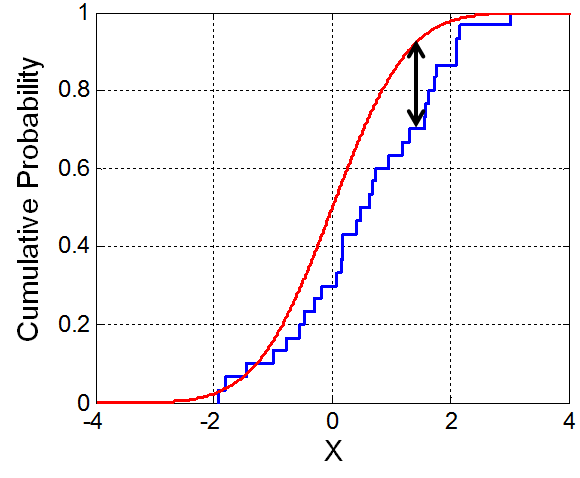
\includegraphics[width=0.45\linewidth]{figs/KS_Example.png}~~~
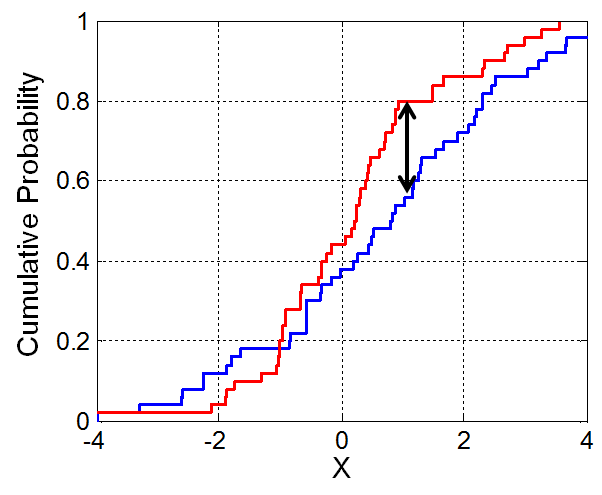
\includegraphics[width=0.45\linewidth]{figs/KS2_Example.png}
\caption{An example Kolmogorov statistic comparing an empirical CDF
with a known, exact CDF (left)  and a Kolmogorov statistic comparing
two empirical CDFs (right). The statistic is indicated by the black,
double-sided arrow. Images taken from 
Wikipedia~\cite{Wiki_kolm}.}
\label{fig:kolm}
\end{figure}

We start with some preliminary definitions. The {\it indicator function}
\index{indicator function} of a subset $A$ of a set $B$ is
the function $\id_A:B\to\{0,1\}$ given by
\begin{equation}
  \id_A(x)=\begin{cases}
    1 & \text{if } x\in A, \\
    0 & \text{otherwise}.
  \end{cases}
\end{equation}
Given some measurements $X_1,...,X_N$, we construct
the {\it empirical CDF} as
\begin{equation}\label{eq:empcdf}
  \bar{F}(x)=\frac{1}{N}\sum_{i=1}^N\id_{[X_i,\infty]}(x),
\end{equation}
where each term counts the number of data less than
or equal to $x$.
The measurements have the same CDF, so at each $x$
we have by the LLN
\begin{equation}\label{eq:empcdfconv}
  \begin{aligned}
  \bar{F}(x)\xrightarrow{\text{P}}
    \ev{\frac{1}{N}\sum_{i=1}^N\id_{[X_i,\infty]}(x)}
    &=\frac{1}{N}\sum_{i=1}^N\ev{\id_{[X_i,\infty]}(x)}\\
    &=\frac{1}{N}\sum_{i=1}^N\pr{X_i\leq x}\\
    &=\frac{1}{N}\sum_{i=1}^NF(x)\\
    &=F(x),
  \end{aligned}
\end{equation}
i.e. $\bar{F}$ is an unbiased, consistent estimator. 
%Before we compute the
%variance, we should note that the variance of each indicator is
%\begin{equation}
%  \sigma^2_\id=\ev{(\id-F)^2}
%              =\ev{\id^2+F^2-2\id F}
%              =F(1-F),
%\end{equation} 
%where we have suppressed the dependence on $x$ and the random variable
%for notational convenience, and utilized $\id^2=\id$. The variance
%of $\bar{F}$ easily follows:
%\begin{equation}
%  \variance\bar{F}(x)=\frac{1}{N^2}\sum_{i=1}^N
%                  \variance{\id_{[X_i,\infty]}(x)}
%                =\frac{1}{N}F(x)\left(1-F(x)\right).
%\end{equation}

The {\it Kolmogorov statistic} is
\begin{equation}
  \Delta\equiv\max_{x\in\R}\left|\bar{F}(x)-F(x)\right|.
\end{equation}
Since $\bar{F}(x)\xrightarrow{\text{P}}F(x)$ for all $x$, it follows
that $\Delta\xrightarrow{\text{P}}0$. An important but surprising
fact about $\Delta$ is that it is {\it distribution free}.
The proof is relatively straightforward and given in
\thmref{thm:koldf}. \thmref{thm:kolprb} gives
the probability that the difference between the empirical and true
CDFs is at least as extreme as what we calculate. This proof is
tedious and not particularly enlightening, so it has been omitted.
If you want to see a proof you can read Berg~\cite{berg_markov_2004},
who attributes it to Birnbaum and Tingey~\cite{birnbaum_one-sided_1951}
and Smirnov~\cite{smirnoff_sur_1939}.
\begin{theorem}{}{koldf}
  All continuous $F$ have the same $\Delta$. 
  \begin{proof}
    We will start with the slightly easier case where $F$ is monotonically
    increasing. In this case, $F^{-1}$ exists and is also monotonically
    increasing. Then by making the variable change $y=F(x)$ we find
    \begin{equation*}
      \begin{aligned}
      \Delta&=\max_{x\in\R}\left|\bar{F}(x)-F(x)\right|\\
            &=\max_{y\in[0,1]}\left|
                \bar{F}\left(F^{-1}(y)\right)-F\left(F^{-1}(y)\right)\right|\\
            &=\max_{y\in[0,1]}\left|
                \bar{F}\left(F^{-1}(y)\right)-y)\right|.
      \end{aligned}
    \end{equation*}
    Let's focus on the $\bar{F}(F^{-1}(y))$ term. We can recast this as
    $$
      \bar{F}\left(F^{-1}(y)\right)
          =\frac{1}{N}\sum_{i=1}^N\id_{[X_i,\infty]}\left(F^{-1}(y)\right)
          =\frac{1}{N}\sum_{i=1}^N\id_{[F(X_i),\infty]}(y),
    $$
    where in the second step we used 
    $F(X)\leq y\Leftrightarrow X\leq F^{-1}(y)$. This shows that the
    empirical CDF of $F^{-1}(y)$ is none other than the empirical CDF 
    of the sample $F(X_1),...,F(X_N)$. But
    $$
      \pr{F(X)\leq t}=\pr{X\leq F^{-1}(t)}=F\left(F^{-1}(t)\right)=t,
    $$
    i.e. the sample is drawn from the uniform distribution in the
    interval $[0,1]$, regardless of what $F$ is. It follows that 
    $\bar{F}\left(F(y)\right)$ is independent of $F$, and hence so 
    is $\Delta$.

    In the case $F$ is not monotonic, the inverse is not guaranteed.
    We define
    $$
      F^+(y)\equiv\min\{x\suchthat F(x)\geq y\}.
    $$
    The important thing is that $F^+(y)\leq z\Leftrightarrow y\leq F(z)$.
    To see this note that
    $$
      F^+(y)\leq z \Rightarrow y\leq F\left(F^+(y)\right)\leq F(z)
    $$
    and
    $$
      y\leq F(z)\Rightarrow F^+(y)\leq F^+\left(F(z)\right)\leq z.
    $$
    The theorem follows by replacing $F^{-1}$ with $F^+$ 
    in the first paragraph.
  \end{proof}
\end{theorem}
\begin{theorem}{}{kolprb}
  Let $D>0$. Then
  $$
    \pr{\Delta>D}=\sum_{k=0}^K{N\choose k}D\left(D+\frac{k}{N}\right)^{k-1}
                   \left(1-D-\frac{k}{N}\right)^{N-k},
  $$
  where $K$ is determined by the condition that $1-D-k/N$ cannot be
  negative. If $N$ is large enough, this probability can be approximated as
  $$
    \pr{\Delta>D}\approx e^{-2ND^2}.
  $$
\end{theorem}

We now have all the ingredients we need to carry out a Kolmogorov test,
and by \thmref{thm:koldf} we are guaranteed it will work, regardless
of the underlying distribution, under the modest assumption that its
CDF is continuous. In practice one can proceed as follows:
\begin{enumerate}
  \item Sort the measurements, then place them into an array $\{X_i\}$.
  \item The $X_i$ are indexed by $i$, so the corresponding empirical CDF 
        is just the array of fractions $\{i/n\}$. For example $X_1\leq X_1$, 
        so $\bar{F}(X_1)=1/N$. Since $X_1,\,X_2\leq X_2$ we have 
        $\bar{F}(X_2)=2/N$.
  \item Compute the exact PDF. For instance if we think the
        data come from $\Gau(x,0,\sigma)$, we can compute the exact CDF
        using \equatref{eq:gaussCDF}; or if we think the data come from the 
        uniform distribution on $[0,1]$, we can just heapsort them.
  \item Determine $\Delta$.
  \item Calculate $\pr{\Delta>D}$ using \thmref{thm:kolprb}.
        If the calculation of the exact probability is slow, you can
        use the approximation, but only if $N$ is big enough, say larger
        than 100 or so.
  \item The underlying assumption is that empirical CDF is an estimator
        for true CDF, so if the probability is below some threshold,
        say 0.05, then this assumption becomes suspect. 
\end{enumerate}

\section{Statistical analysis of time series}

Once we get into lattice calculations, we are going to analyze
Markov chains, which we'll discuss in \chref{ch:MCMC}. There
we'll consider a {\it time series}\index{time series} of $N$
measurements
\begin{equation}
\{X_1, ..., X_N\}. 
\end{equation}
The idea of a time series is that each measurement
$X_i$ is in principle somehow correlated with $X_{i-1}$.
For instance one can consider a time series of temperature
measurements in a city. In our case, we'll generate a time
series of space-time configurations, where each configuration
is generated based on the preceding one.

\subsection{Autocorrelation}

In principle each element of this sample is drawn
from a PDF with mean $\ev{X_i}=\ev{X}=\hat{x}$ and variance 
$\sigma^2=\ev{(X_i-\hat{x})^2}$, i.e. they all have the same mean
and variance. Unbiased estimators for the mean and variance are
\begin{equation}\label{eq:umv}
  \bar{X}=\frac{1}{N}\sum_{i=1}^N X_i
  ~~~~\text{and}~~~~
  \bar{\sigma}^2=\frac{1}{N-1}\sum_{i=1}^N (X_i-\bar{X})^2.
\end{equation}
The variance of the random variable $\bar{X}$ is
\begin{equation}\label{eq:tsvar}
  \sigma^2_{\bar{X}}=\ev{(\bar{X}-\hat{x})^2}
                    =\frac{1}{N^2}\left(\sum_{i\neq j}\ev{X_iX_j}
                     +N\ev{X^2}\right)-\hat{x}^2.
\end{equation}
In the case that the measurements are effectively uncorrelated, the expected values
factorize, and we obtain
\begin{equation}
  \sigma^2_{\bar{X}}=\sigma^2/N
\end{equation}
in agreement with the CLT. But in practice measurement
$i+1$ is often correlated with measurement $i+t$. 
To measure this we draw inspiration from 
definition \eqref{dfn:cor}. 
The {\it autocovariance}\index{autocovariance} between measurements 
$X_i$ and $X_{i+t}$ is
  \begin{equation}\label{dfn:acov}
    c(X_i,X_{i+t})\equiv\ev{(X_i-\hat{x})(X_{i+t}-\hat{x})}
     =\ev{X_iX_{i+t}}-\ev{X_i}\ev{X_{i+t}},
  \end{equation}
For a Markov process in equilibrium, the autocovariance depends only on 
the separation $t$, so we define $c(t)\equiv c(X_i,X_{i+t})$. Finally note that
$c(0)=\sigma^2$, which motivates the definition of the {\it autocorrelation}
\index{autocorrelation}
\begin{equation}\label{dfn:acor}
  \gamma(t)\equiv\frac{c(t)}{\sigma^2}.
\end{equation}
The autocorrelation decays in $t$ as a sum of exponentials. I don't
know why this is true, and I couldn't find a reference, but this is what
everybody says. Assuming this is the case we can write
\begin{equation}
  \gamma(t)=A_\text{exp}\,e^{-t/\tau_\text{exp}}
            +\sum_{i=1}^\infty A_i\,e^{-t/\tau_i},
\end{equation}
where the $A$s are constants and we have picked out the leading
exponential behavior; i.e. for all $i$
\begin{equation}\index{autocorrelation time!exponential}
  \tau_\text{exp}>\tau_i.
\end{equation}
$\tau_\text{exp}$ is called the {\it exponential autocorrelation time}.

Plugging definition \eqref{dfn:acov} into \equatref{eq:tsvar} we have 
\begin{equation}
  \sigma^2_{\bar{X}}=\frac{1}{N^2}\sum_{i,j}c(X_i,X_j).
\end{equation}
In the last sum, $|i-j|=0$ occurs $N$ times, and $|i-j|=t$ occurs
$2(N-t)$ times. Note $1\leq t\leq N-1$. Therefore
\begin{equation}
  \sigma^2_{\bar{X}}=\frac{1}{N^2}
    \left(N\,c(0)+2\sum_{t=1}^{N-1}(N-t)c(t)\right).
\end{equation}
Finally we use $c(0)=\sigma^2$ to find
\begin{equation}\label{eq:IAC}
  \sigma^2_{\bar{X}}
    =\frac{\sigma^2}{N}\left(1+2\sum_{t=1}^{N-1}\left(1-\frac{t}{N}\right)
     \gamma(t)\right)
    \equiv\frac{\sigma^2}{N}\tau_\text{int}.
\end{equation}
The quantity
\begin{equation}\label{dfn:IAC}\index{autocorrelation time!integrated}
  \tauint=\left(1+2\sum_{t=1}^{N-1}\left(1-\frac{t}{N}\right)
   \gamma(t)\right)
\end{equation}
is called the {\it integrated autocorrelation time}.

From \equatref{eq:IAC} we see that $\tauint$ is just the ratio between the
estimated variance of the sample mean and what this variance would have been 
if the data were uncorrelated. 

In practice, we often don't know the true mean $\hat{x}$ of the time series.
Therefore along the lines of \equatref{eq:umv}, we construct an unbiased
estimator of the autocovariance
\begin{equation}
  \bar{c}(t)=\frac{N}{(N-1)(N-t)}
    \sum_{i=1}^{N-t}(X_i-\bar{X})(X_{i+t}-\bar{X}),
\end{equation}
where it is the factor $N/(N-1)$ that removes the bias, just as before.
Also in most situations we work in the limit where $N$ is large. In this
limit, we can construct an estimator for $\tau_\text{int}$ by
\begin{equation}\label{eq:IACest}
  \bar{\tau}_\text{int}(n)=1+2\sum_{t=1}^n\bar{\gamma}(t),
\end{equation}
where $n<N$. To understand the above estimator look at definition
\eqref{dfn:IAC}. When $t$ is small, $1-t/N\approx 1$. Large $t$ terms
are doubly suppressed by the exponential decay of $\gamma(t)$ and
by $1-t/N\approx 0$. If the estimator still makes you uncomfortable,
note that in the overly simplistic case where
$\gamma(t)$ has only one exponential term, one can prove
\begin{equation}
  \lim_{N\to\infty}\tau_\text{int}=1+2\sum_{t=1}^\infty\gamma(t),
\end{equation}
which parallels \equatref{eq:IACest} more closely. To construct a final
estimator for $\tauint$, one looks for a window in $n$ for which
\equatref{eq:IACest} becomes roughly independent of $n$. This serves
as the final $\bar{\tau}_\text{int}$.

\subsection{Correlation between two series}


Consider now two series with measurements indicated by $X_i$ and $Y_i$;
we assume the series are of the same length. Again drawing
inspiration from definition \eqref{dfn:cor}, we define the
{\it Pearson correlation coefficient}\footnote{This is the same number that gets 
delivered in Excel when you fit a line.}
as\index{correlation!Pearson}
\begin{equation}
r\equiv
\frac{\sum_{i=1}^n\left(X_i-\bar{X}\right)\left(Y_i-\bar{Y}\right)}{\sqrt{\sum_{j=1}^n\left(X_j-\bar{X}\right)^2}
\sqrt{\sum_{k=1}^n\left(Y_k-\bar{Y}\right)^2}}.
\end{equation}
If the series are not correlated, you would expect a deflection of $X_i$
above its mean would be roughly as likely as a deflection of $Y_i$
below its mean, and hence $r\approx0$. The denominator normalizes this
quantity so that it falls in the range $r\in[-1,1]$.

\section{The Bayesian approach}\label{sec:bayes}

The probability assignment rule \equatref{eq:freqdef} effectively summarizes 
the frequentist\index{frequentist approach} interpretation of probability. Here we
will describe another interpretation, the {\it Bayesian}\index{Bayesian
approach} interpretation. An excellent introduction to this approach
to probability theory can be found in, e.g. Ref.~\cite{sivia_data_2006}.

To motivate this approach, I want to share an example of an interesting false
signal from experimental particle physics. In this context, we are often tasked
with the challenge of discerning a signal within some background distribution.
One can use a variety of statistics\footnote{For instance the Kolmogorov
statistic of \secref{sec:kolm}.} to compute the probability that the observed
distribution is consistent with the background. To help protect against
reporting a false signal, particle physicists have decided to place the
discovery threshold at 5$\sigma$, which according to \tabref{tab:normal}
yields a probability of about $5.7\times10^{-7}$. In 2004, physicists
reported the discovery of a pentaquark\footnote{This is a
5-quark\index{pentaquark} bound state.} with a probability of about
$4\times10^{-8}$ of being a genuine signal, well beyond the
5$\sigma$ threshold~\cite{aktas_evidence_2004}. This pentaquark could
not be found by subsequent groups; Ref.~\cite{rossi_tetra-quarks_2021}
includes a nice summary of the matter.

So what went wrong? Were we just really unlucky? In fact this signal was due to
a mistake in the analysis. Does this mean the people who calculated the
probability didn't know what they were doing? On the contrary, the probability
was calculated under the assumption that the analysis was correct; in other
words, it was calculated in the context of the information they had available at
the time.

This is the essence of the Bayesian approach: it generalizes the notion of a 
probability to a degree of belief. If you like, you can view it as an attempt to
be more honest about assumptions are made or what knowledge goes into a
calculation. This knowledge is summarized by probability distributions called
{\it priors}\index{prior}.

\subsection{Rules for consistent reasoning}\label{sec:consistentReasoning}

In 1946, Cox thought about how to quantitatively assign likelihoods to
statements about the word in a consistent manner~\cite{cox_probability_1946}. 
The idea is that one wants to
take statements like ``The sun will rise tomorrow" or ``Jerry attacked Tom" and
assign real numbers to them such that the real number is higher for the
statement in whose truth one has greater confidence.
In general one considers statements $A$ and $B$ and assigns them
real numbers $\pr{A}$ and $\pr{B}$, which defines our 
{\it probabilities}\index{probability}. 
Cox showed that consistency is ensured
if the real numbers satisfy
\begin{equation}\begin{aligned}
\pr{A\given I}+\pr{\neg A\given I}&=1,\\
\pr{A\wedge B\given I}&=\pr{A\given B\wedge I}\pr{B\given I},\\
\pr{\text{true}}&=1,\\
\pr{\text{false}}&=0.
\end{aligned}\end{equation}
The vertical bar $|$ in this context means ``given", i.e. everything to the
right of this bar is taken to be true. In each case we include this symbol $I$
to indicate some possible background information that is known ahead of time.
The first of these two equations is sometimes called the {\it sum
rule}\index{rule!sum} while the second is sometimes called the {\it product
rule}\index{rule!product}. It can be used to relate conditional probabilities
in the following manner.

\index{Bayes's Theorem} 
\begin{theorem}{Bayes's Theorem}{} 
$$
\pr{A\given B\land I}=\frac{\pr{B\given A\land I}\pr{A\given I}}{\pr{B\given I}}
$$
  \begin{proof}
  From the product rule we have both
\begin{equation*}\begin{aligned}
\pr{A\wedge B\given I}&=\pr{A\given B\wedge I}\pr{B\given I},\\
\pr{B\wedge A\given I}&=\pr{B\given A\wedge I}\pr{A\given I}.
\end{aligned}\end{equation*}
  Since the statements $A\land B$ and $B\land A$ are exactly the same, we can
eliminate the LHS and solve for $\pr{A\given B\land I}$.
  \end{proof}
\end{theorem}

This relation between the conditional probabilities is useful especially in the
context of data analysis, for if we replace $A$ by ``model" and $B$ by ``data",
we get 
\begin{equation}
\pr{\text{model}\given \text{data}\land I}
=\frac{\pr{\text{data}\given \text{model}\land I}\pr{\text{model}\given I}}{\pr{\text{data}\given
I}}.
\end{equation}
In particular, in the context of analyzing data, the LHS is what is difficult to
ascertain. One may have a bunch of competing ways of looking at things and
desires the way of looking at things that is, given the information $I$ at hand,
the most probable. The LHS is called the {\it posterior}\index{posterior}
probability. It is related to the {\it likelihood}\index{likelihood} that one
would find these data given the hypothesis, $\pr{\text{data}\given
\text{model}\land I}$ as well as the {\it prior}\index{prior}
probability $\pr{\text{model}\given I}$, which represents our state of
knowledge about the model before analyzing the data. The denominator term,
$\pr{\text{data}\given I}$ is called\footnote{It is also sometimes called
the {\it prior predictive}\index{prior!predictive} or the 
{\it marginal likelihood}\index{likelihood!marginal}.} 
the {\it evidence}\index{evidence}. 

We note one more useful property of conditional probabilities, that
\begin{equation}
\pr{A\land I}=\int_{-\infty}^\infty \dd{B} f(A\given B\land I),
\end{equation}
where $f$ is a PDF to be interpreted like in \secref{sec:probprelim}.
This is the statement that if $A$ is conditional on $B$, I can arrive at a
statement involving $A$ alone by exhaustively integrating over all possible
outcomes for $B$. This process is known\footnote{When we do this in a physics
context instead of a statistical context, we usually say we are ``integrating
out" $B$.} as {\it marginalization}\index{marginalization}.

Marginalization is useful in the same way integrating out is useful: If we know
e.g. that a model contains some explicit dependence on some parameter $\lambda$
but we don't know what it is, the exhaustive integration lets us make statements
independent of it. In the context of statistical analysis, such quantities are
often called {\it nuisance parameters}\index{nuisance parameter}.

\subsection{Interpreting probabilities}

Perhaps the nicest characteristic of the frequentist approach is that it
provides a clear interpretation of a probability like 0.98; in particular we
imagine some ensemble of 100 experiments or universes and claim that, on
average, our event of interest would occur 98 times. In the Bayesian case, by
contrast, a probability as we have presented it in
\secref{sec:consistentReasoning} has no such a priori interpretation. Instead it
is a degree of confidence that we demand should have certain properties, for
instance that if $\pr{A}>\pr{B}$ then we think that $A$ is more ``likely to
occur" than $B$. For this reason, some authors view it as an extension of
ordinary logic. Which is preferable for probability assignment?

To begin with, I want to list a couple drawbacks of the frequentist approach.
The first is that this ensemble interpretation is not always reasonable. Cox
gives an example from number theory~\cite{cox_probability_1946} that should hold
for one of the integers 4, 5, 6, 7, or 8. A mathematician surmises that
4 is the ``most likely". What would it mean to imagine an ensemble in this case,
that is, what kind of statistical spread can you imagine for something that,
when determined, gives a unique, unambiguous result?
The second kind of drawback concerns the example of the pentaquark given at the
beginning, namely that it ignores the role of limited information. Every
probability in a Bayesian context is explicitly written as conditional on
whatever information is available at the time. This is a subtle point, but its
corollary is important: The frequentist computation of the discovery probability 
yields a false statement. The Bayesian computation, which would arrive at the same 
number, would yield a true statement, since it is conditional on the limited
understanding of that experimental analysis. To put it another way, the
frequentist approach strives to yield an objective number independent of all
context, while the Bayesian approach softens this goal to a demand that
observers with the same knowledge obtain the same number.

I found myself still somewhat uncomfortable with the loss of the ensemble
interpretation of probabilities, because it let me say unambiguously ``this is
what 0.98 means". This discomfort can be largely resolved by approaching this
superficially alien way of looking at probabilities in a similar manner as when
one first becomes comfortable with special relativity or quantum mechanics,
specifically by noting that the Bayesian interpretation reduces to the
frequentist one in familiar cases. For example when $I$ represents the
information that one rolls an ideal, fair die, one can again imagine the
ensemble of die throws, and one obtains the same number as the frequentist does.
Therefore the observer hasn't lost any interpreting power; on the contrary, the 
observer gains the ability to assign numbers representing degrees of certainty to
situations where the ensemble interpretation is useless.


\subsection{Assigning probabilities}


Now that we've thought about what the probabilities mean in the Bayesian
framework, we need a way to assign them; in the frequentist framework, it was
sufficient to use ratios of set sizes, but now this assignment isn't automatic.
 

\bibliographystyle{unsrtnat}
\bibliography{bibliography}
